\documentclass{standalone}
\usepackage{../../../../preamble_formulas}
\begin{document}
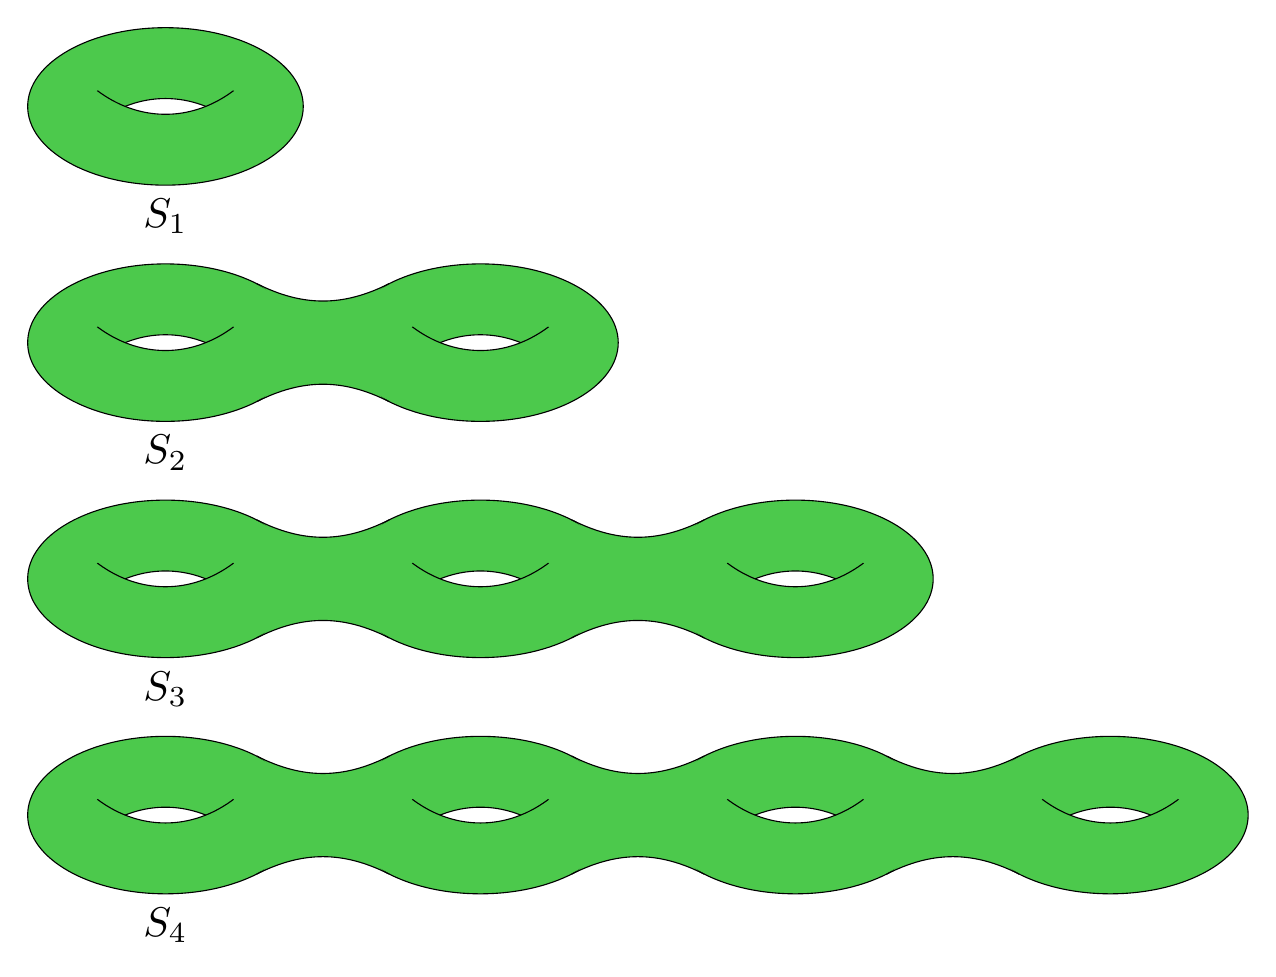
\begin{tikzpicture}
  \def\a{2}
  \def\b{0.5}
  \def\manifold#1#2#3#4{
    \draw[fill=#4] (#1,#2) ellipse (1.75 and 1);
    \begin{scope}
      \clip (#1,#2+2.2) ellipse (1.75 and 2.3);
      \draw[fill=white] (#1,#2-2.2) ellipse (1.75 and 2.3);
    \end{scope}
    \begin{scope}
      \clip (#1,#2-1.8) ellipse (1.75 and 2.3);
      \draw (#1,#2+2.2) ellipse (1.75 and 2.3);
    \end{scope}
    \node[scale=1.5] at (#1,-1.4+#2){#3};
  }
  \def\union#1#2{
    \fill[green!70!black!70]
    (#1+-0.8425,#2+0.75) to[out=-26.746,in=180+26.746]
    (#1+0.8425,#2+0.75) to[out=180+26.746,in=180-26.746]
    (#1+0.8425,#2+-0.75) to[out=180-26.746,in=26.746]
    (#1+-0.8425,#2+-0.75) to[out=26.746,in=-26.746]
    (#1+-0.8425,#2+0.75);
    \draw[black]
    (#1+-0.8425,#2+0.75) to[out=-26.746,in=180+26.746]
    (#1+0.8425,#2+0.75)
    (#1+0.8425,#2+-0.75) to[out=180-26.746,in=26.746]
    (#1+-0.8425,#2+-0.75);
  }
  \useasboundingbox (-\a-1.75,-7.7) rectangle (5*\a+1.75,4);

  %%% S1
  \manifold{-\a}{3}{$S_1$}{green!70!black!70}

  %%% S2
  \manifold{-\a}{0}{$S_2$}{green!70!black!70}
  \manifold{\a}{0}{}{green!70!black!70}
  \union{0}{0}

  %%% S3
  \manifold{-\a}{-3}{$S_3$}{green!70!black!70}
  \manifold{\a}{-3}{}{green!70!black!70}
  \manifold{3*\a}{-3}{}{green!70!black!70}
  \union{0}{-3}
  \union{2*\a}{-3}

  %%% S3
  \manifold{-\a}{-6}{$S_4$}{green!70!black!70}
  \manifold{\a}{-6}{}{green!70!black!70}
  \manifold{3*\a}{-6}{}{green!70!black!70}
  \manifold{5*\a}{-6}{}{green!70!black!70}
  \union{0}{-6}
  \union{2*\a}{-6}
  \union{4*\a}{-6}
\end{tikzpicture}

\end{document}